\newpage
\section{Questão 12-33}

\begin{figure}[H]
	\centering
	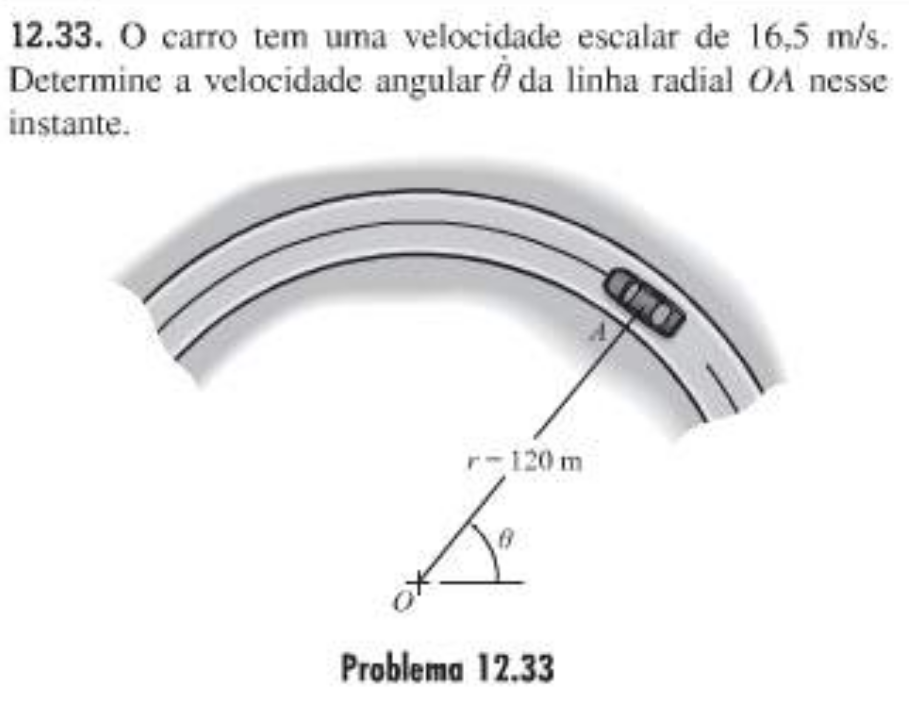
\includegraphics[width=.7\linewidth]{fundamentais/12-33.png}
	\caption{Comando da questão 12-33}\label{fig:12-33}
\end{figure}

Nesta questão, analisamos o movimento de uma partícula em uma trajetória circular com raio \(r = 120 \, \text{m}\) e velocidade escalar \(v = 16.5 \, \text{m/s}\). Determinamos a velocidade angular \(\dot{\theta}\) da partícula.

\subsection*{Cálculo da Velocidade Angular}
A relação entre a velocidade angular \(\dot{\theta}\) e a velocidade escalar \(v\) em uma trajetória circular é dada por:
\[
\dot{\theta} = \frac{v}{r},
\]
onde:
\begin{itemize}
    \item \(\dot{\theta}\): Velocidade angular (em rad/s);
    \item \(v\): Velocidade escalar (em m/s);
    \item \(r\): Raio da trajetória circular (em m).
\end{itemize}

\subsection*{Substituição dos Valores Numéricos}
Substituímos os valores \(v = 16.5 \, \text{m/s}\) e \(r = 120 \, \text{m}\) na equação:
\[
\dot{\theta} = \frac{16.5}{120}.
\]

Simplificando:
\[
\dot{\theta} \approx 0.138 \, \text{rad/s}.
\]

\subsection*{Resultado Final}
A velocidade angular da partícula é:
\[
\dot{\theta} \approx 0.138 \, \text{rad/s}.
\]
